\documentclass[plain]{beamer}
\setbeamertemplate{navigation symbols}{}
\setbeamercolor{frametitle}{fg=black}
\setbeamercolor{title}{fg=black}

\usepackage[ngerman]{babel}
\usepackage{graphics}
\usepackage{keystroke}
\usepackage{todonotes}

\newcommand{\prefix}{\Ctrl+\keystroke{b}}
\newcommand{\tmux}{\texttt{tmux}}
\newcommand{\demoslide}{\begin{frame}
  \center \huge DEMO
\end{frame}}

\title{\huge \tmux{}}
\author{Max Schik}

\begin{document}

\begin{frame}
  \titlepage
\end{frame}

\begin{frame}
  Ihr seid hier weil ihr ...
  \begin{itemize}
    \item ... \tmux{} noch nicht kennt, es sich aber interessant anhört
    \item ... \tmux{} bereits verwendet, aber gerne noch etwas neues lernen möchtet
    \item ... euch nicht für ML interessiert
  \end{itemize}
\end{frame}

\begin{frame}
  \begin{columns}[onlytextwidth,T]
    \column{\dimexpr\linewidth-30mm-5mm}
    Wer ist eigentlich dieser \tmux{}?
    \begin{itemize}
      \item \textbf{T}erminal \textbf{MU}ltiple\textbf{X}er
      \item aus dem Jahre 2007, entwickelt von Nicholas Marriott
      \item steht unter ISC Lizenz (also quasi BSD/MIT)
      \item Wird immer noch weiterentwickelt
    \end{itemize}
    \column{30mm}
    
\includegraphics[width=\textwidth]{imgs/Tmux_logo.png}
  \end{columns}
\end{frame}

\begin{frame}
  Und was kann dieses \tmux{}?
  \begin{itemize}
    \item Mehrere Terminals in einem Fenster (auch ohne X-Kellner!)
    \item Kollaboratives Arbeiten
    \item Sitzung ist persistent, auch wenn die Verbindung mal abschmiert
    \item Ermöglicht Kopieren/Einfügen/Zurückscrollen ohne Maus
  \end{itemize}
\end{frame}

\demoslide{}

\begin{frame}
  Wo kriegt man denn dieses \tmux{} her?
  \begin{itemize}
    \item unter Ubuntu: \texttt{sudo apt install tmux}
    \item für die Profis: \url{https://github.com/tmux/tmux}
  \end{itemize}
\end{frame}

\demoslide

\begin{frame}
  \begin{itemize}
    \item \tmux{} starten: \texttt{tmux}
    \item sich von einer \tmux{} Sitzung ablösen: \prefix, \keystroke{d}
    \item sich wieder an eine Sitzung anhängen: \texttt{tmux a[ttach]}
    \item Sitzung töten: \prefix, \keystroke{:}, \texttt{kill-session}
    \item Feld töten: \prefix, \keystroke{x}, \keystroke{y}
    \item vertikaler Unterteilung: \prefix, \keystroke{\%}
    \item horizontaler Unterteilung: \prefix, \keystroke{``}
    \item Feld wechseln: \prefix, \keystroke{o} \\ oder \prefix, \textit{Pfeiltasten}
    \item Sitzung wechseln: \prefix, \keystroke{s}
    \item Es gibt noch mehr aber sie werden nicht besser
  \end{itemize}
\end{frame}

\begin{frame}
  Muss ich Lack trinken um diese Tastenkombinationen zu verstehen?
  \begin{itemize}
    \item Ja
  \end{itemize}
  \center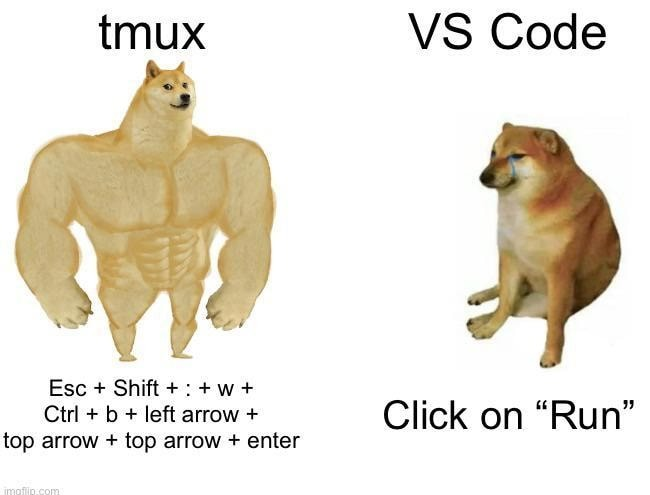
\includegraphics[width=0.7\textwidth]{imgs/keybinds_meme.jpg}
\end{frame}

\begin{frame}
  \begin{itemize}
    \item Die meisten Tastenkombinationen in \tmux{} fangen mit dem \textbf{Prefix} an
    \item standardmäßig ist das \prefix
    \item man könnte argumentieren dass die Voreinstellungen ziemlich unintuitiv sind
    \item das kann man sich allerdings ganz einfach umstellen
  \end{itemize}
\end{frame}

\begin{frame}
  \begin{itemize}
    \item \tmux{} lässt sich über eine Konfigurationsdatei anpassen
    \item normalerweise findet man die unter \texttt{\$HOME/.tmux.conf}
    \item Konfiguration laden mit \texttt{tmux source-file \$HOME/.tmux.conf}
  \end{itemize}
\end{frame}

\begin{frame}
  \begin{itemize}
    \item erstmal den Prefix auf etwas weniger schmerzhaftes legen: \\
    \texttt{unbind C-b \\
            set-option -g prefix C-space \\
            bind-key C-space send-prefix}

    \item Navigation zwischen Feldern weniger schmerzhaft machen: \\
    \texttt{bind-key -n C-h select-pane -L \\
            bind-key -n C-j select-pane -D \\
            bind-key -n C-k select-pane -U \\
            bind-key -n C-l select-pane -R}

    \item Mausunterstützung:\\
    \texttt{set -g mouse on}
    \item (Optional) Farben reparieren:\\
    \texttt{set -g default-terminal "tmux-256color"\\
            set -ag terminal-overrides ",xterm-256color:RGB"}
  \end{itemize}
\end{frame}

\demoslide

\begin{frame}
  \center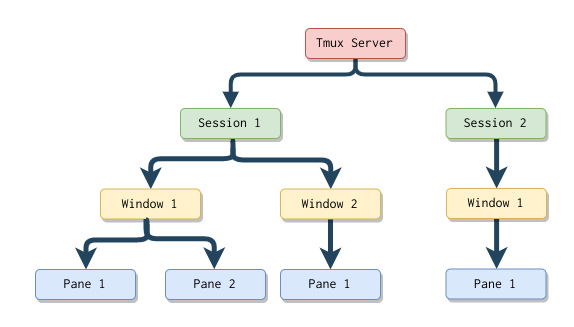
\includegraphics[width=\textwidth]{imgs/tmux-working-diagram.jpg}
\end{frame}

\begin{frame}
  Tmux lässt sich wunderbar skripten
  \begin{itemize}
    \item \texttt{tmux [COMMAND] -t [SESSION:WINDOW.PANE]} kann benutzt werden um befehle an \tmux{}
      Sitzungen zu schicken
    \item z.Bsp. \texttt{tmux split-window -t 0} unterteilt die Sitzung mit Id 0
    \item Man kann sich damit ganz schnell Skripte schreiben die einem ein \tmux{} setup bereitstellen
  \end{itemize}
\end{frame}

\demoslide{}

\begin{frame}
\begin{itemize}
  \item \texttt{catmux} (\url{https://github.com/fmauch/catmux}) vereinfacht das erstellen von
    vorgefertigten Sitzungen (sehr praktisch für ROS)
  \item \texttt{vim-tmux-navigator} (\url{https://github.com/christoomey/vim-tmux-navigator}) ist
    sehr gut für Leute die Vim verwenden
\end{itemize}
\end{frame}

\begin{frame}
  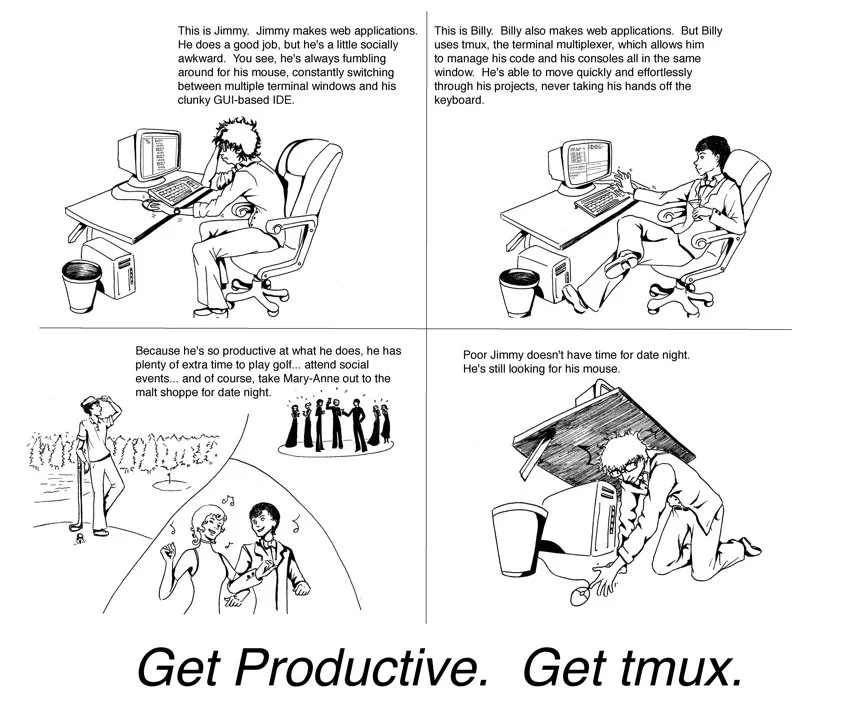
\includegraphics[width=\textwidth]{imgs/tmux_final_meme.png}
\end{frame}

\end{document}

